%%%%%%%%%%%%%%%%%%%%%%%%%%%%%%%%%%%%%
%% Supporting Information
%% (Optional)
%%%%%%%%%%%%%%%%%%%%%%%%%%%%%%%%%%%%%
% OVERVIEW
%
% Please note that all supporting information will be peer reviewed with your manuscript.
% In general, the purpose of the supporting information is to enable
% authors to provide and archive auxiliary information such as data
% tables, method information, figures, video, or computer software,
% in digital formats so that other scientists can use it.

% The key criteria are that the data:
% 1. supplement the main scientific conclusions of the paper but are not essential to the conclusions (with the exception of
%    including data so the experiment can be reproducible);
% 2. are likely to be usable or used by other scientists working in the field;
% 3. are described with sufficient precision that other scientists can understand them, and
% 4. are not exe files.
%

% All Supporting text and figures should be included in this document.

% Data sets, large tables, movie files,
% and audio files should be uploaded separately, following AGU naming
% conventions. Include their captions in this document and list the
% file name with the caption. You will be prompted to upload these
% files on the Upload Files tab during the submission process, using
% file type “Supporting Information (SI)”

\documentclass[draft]{agujournal}

% Please type in the journal name: \journalname{<Journal Name>}
% ie,
\journalname{JGR-Atmospheres}

\DeclareGraphicsExtensions{.pdf, .png, .jpg, .eps}
\graphicspath{ {./figs/} }
%% Choose from this list of Journals:
%
% Journal of Geophysical Research
% JGR-Biogeosciences
% JGR-Earth Surface
% JGR-Planets
% JGR-Solid Earth
% JGR-Space Physics
% Global Biochemical Cycles
% Geophysical Research Letters
% Paleoceanography
% Radio Science
% Reviews of Geophysics
% Tectonics
% Space Weather
% Water Resource Research
% Geochemistry, Geophysics, Geosystems
% Journal of Advances in Modeling Earth Systems (JAMES)
% Earth's Future
% Earth and Space Science

\begin{document}

%% This command needs article title as argument to \supportinginfo{}:
\supportinginfo{On the relationship between Arctic fall season precipitation and minimum sea ice extent}

\authors{Joseph Hamman\affil{1} ,
         Bart Nijssen\affil{1},
         Andrew Roberts\affil{2},
         John Cassano\affil{3}}

\affiliation{1}{Department of Civil \& Environmental Engineering,
University of Washington, Seattle, WA, USA.}
\affiliation{2}{Department of Oceanography, Naval Postgraduate School,
Monterey, CA, USA.}
\affiliation{3}{Cooperative Institute for Research in Environmental Sciences,
and Department of Atmospheric and Oceanic Sciences, University of Colorado, Boulder, Colorado}

%% Corresponding Author
%(include name and email addresses of the corresponding author.  More
%than one corresponding author is allowed in this Word file and for
%publication; but only one corresponding author is allowed in our
%editorial system.)

\correspondingauthor{Bart Nijssen}{nijssen@uw.edu}

%% ------------------------------------------------------------------------ %%
%
%  TEXT
%
%% ------------------------------------------------------------------------ %%

\section{Figures}

\clearpage
\begin{figure}
    \centering
    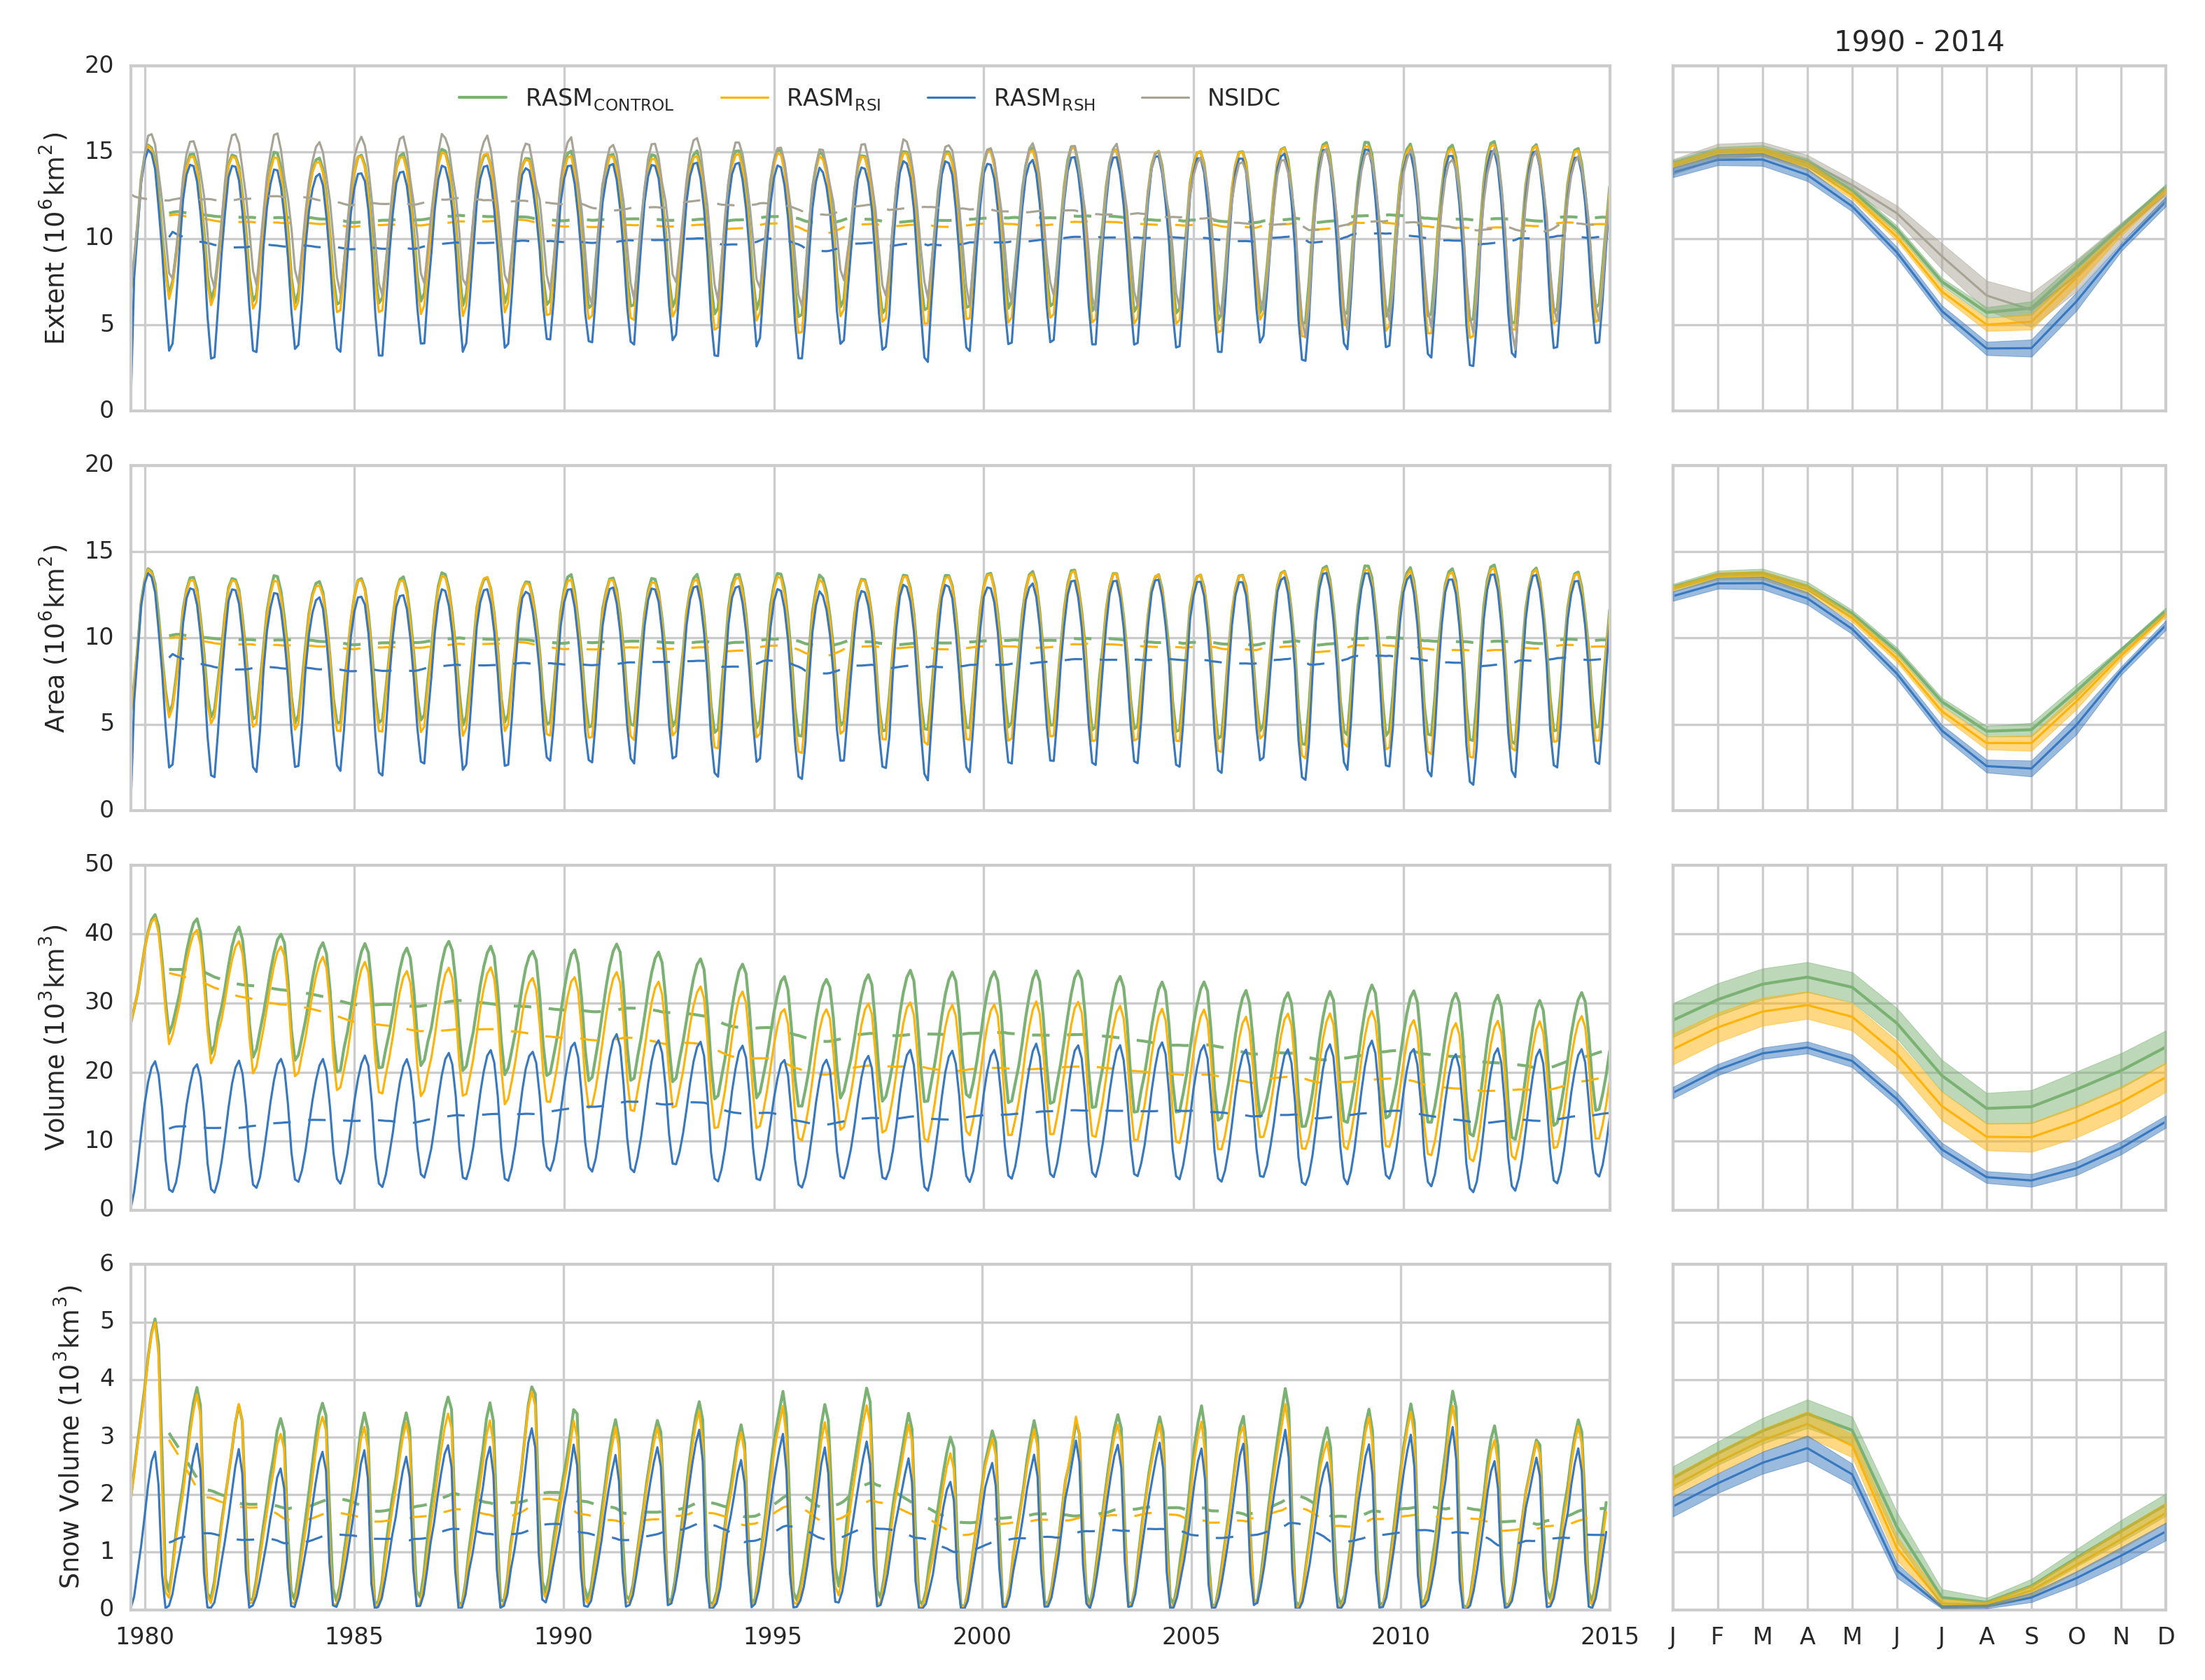
\includegraphics[width=16cm,keepaspectratio]{sea_ice_timeseries}
    \caption{Timeseries of RASM simulated sea ice extent, area, volume, and snow volume. Time period: 1979-2014.}
    \label{fig:sea_ice_ts_sup}
\end{figure}

\clearpage
\begin{figure}
    \centering
    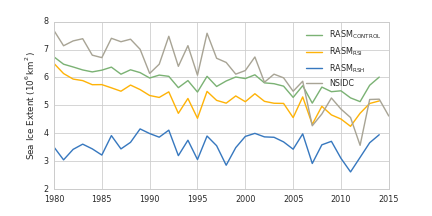
\includegraphics[width=16cm,keepaspectratio]{sea_ice_min_timeseries}
    \caption{Timeseries of RASM simulated minimum annual sea ice extent. Time period: 1979-2014.}
    \label{fig:sea_ice_min_ts_sup}
\end{figure}

\clearpage
\begin{figure}
    \centering
    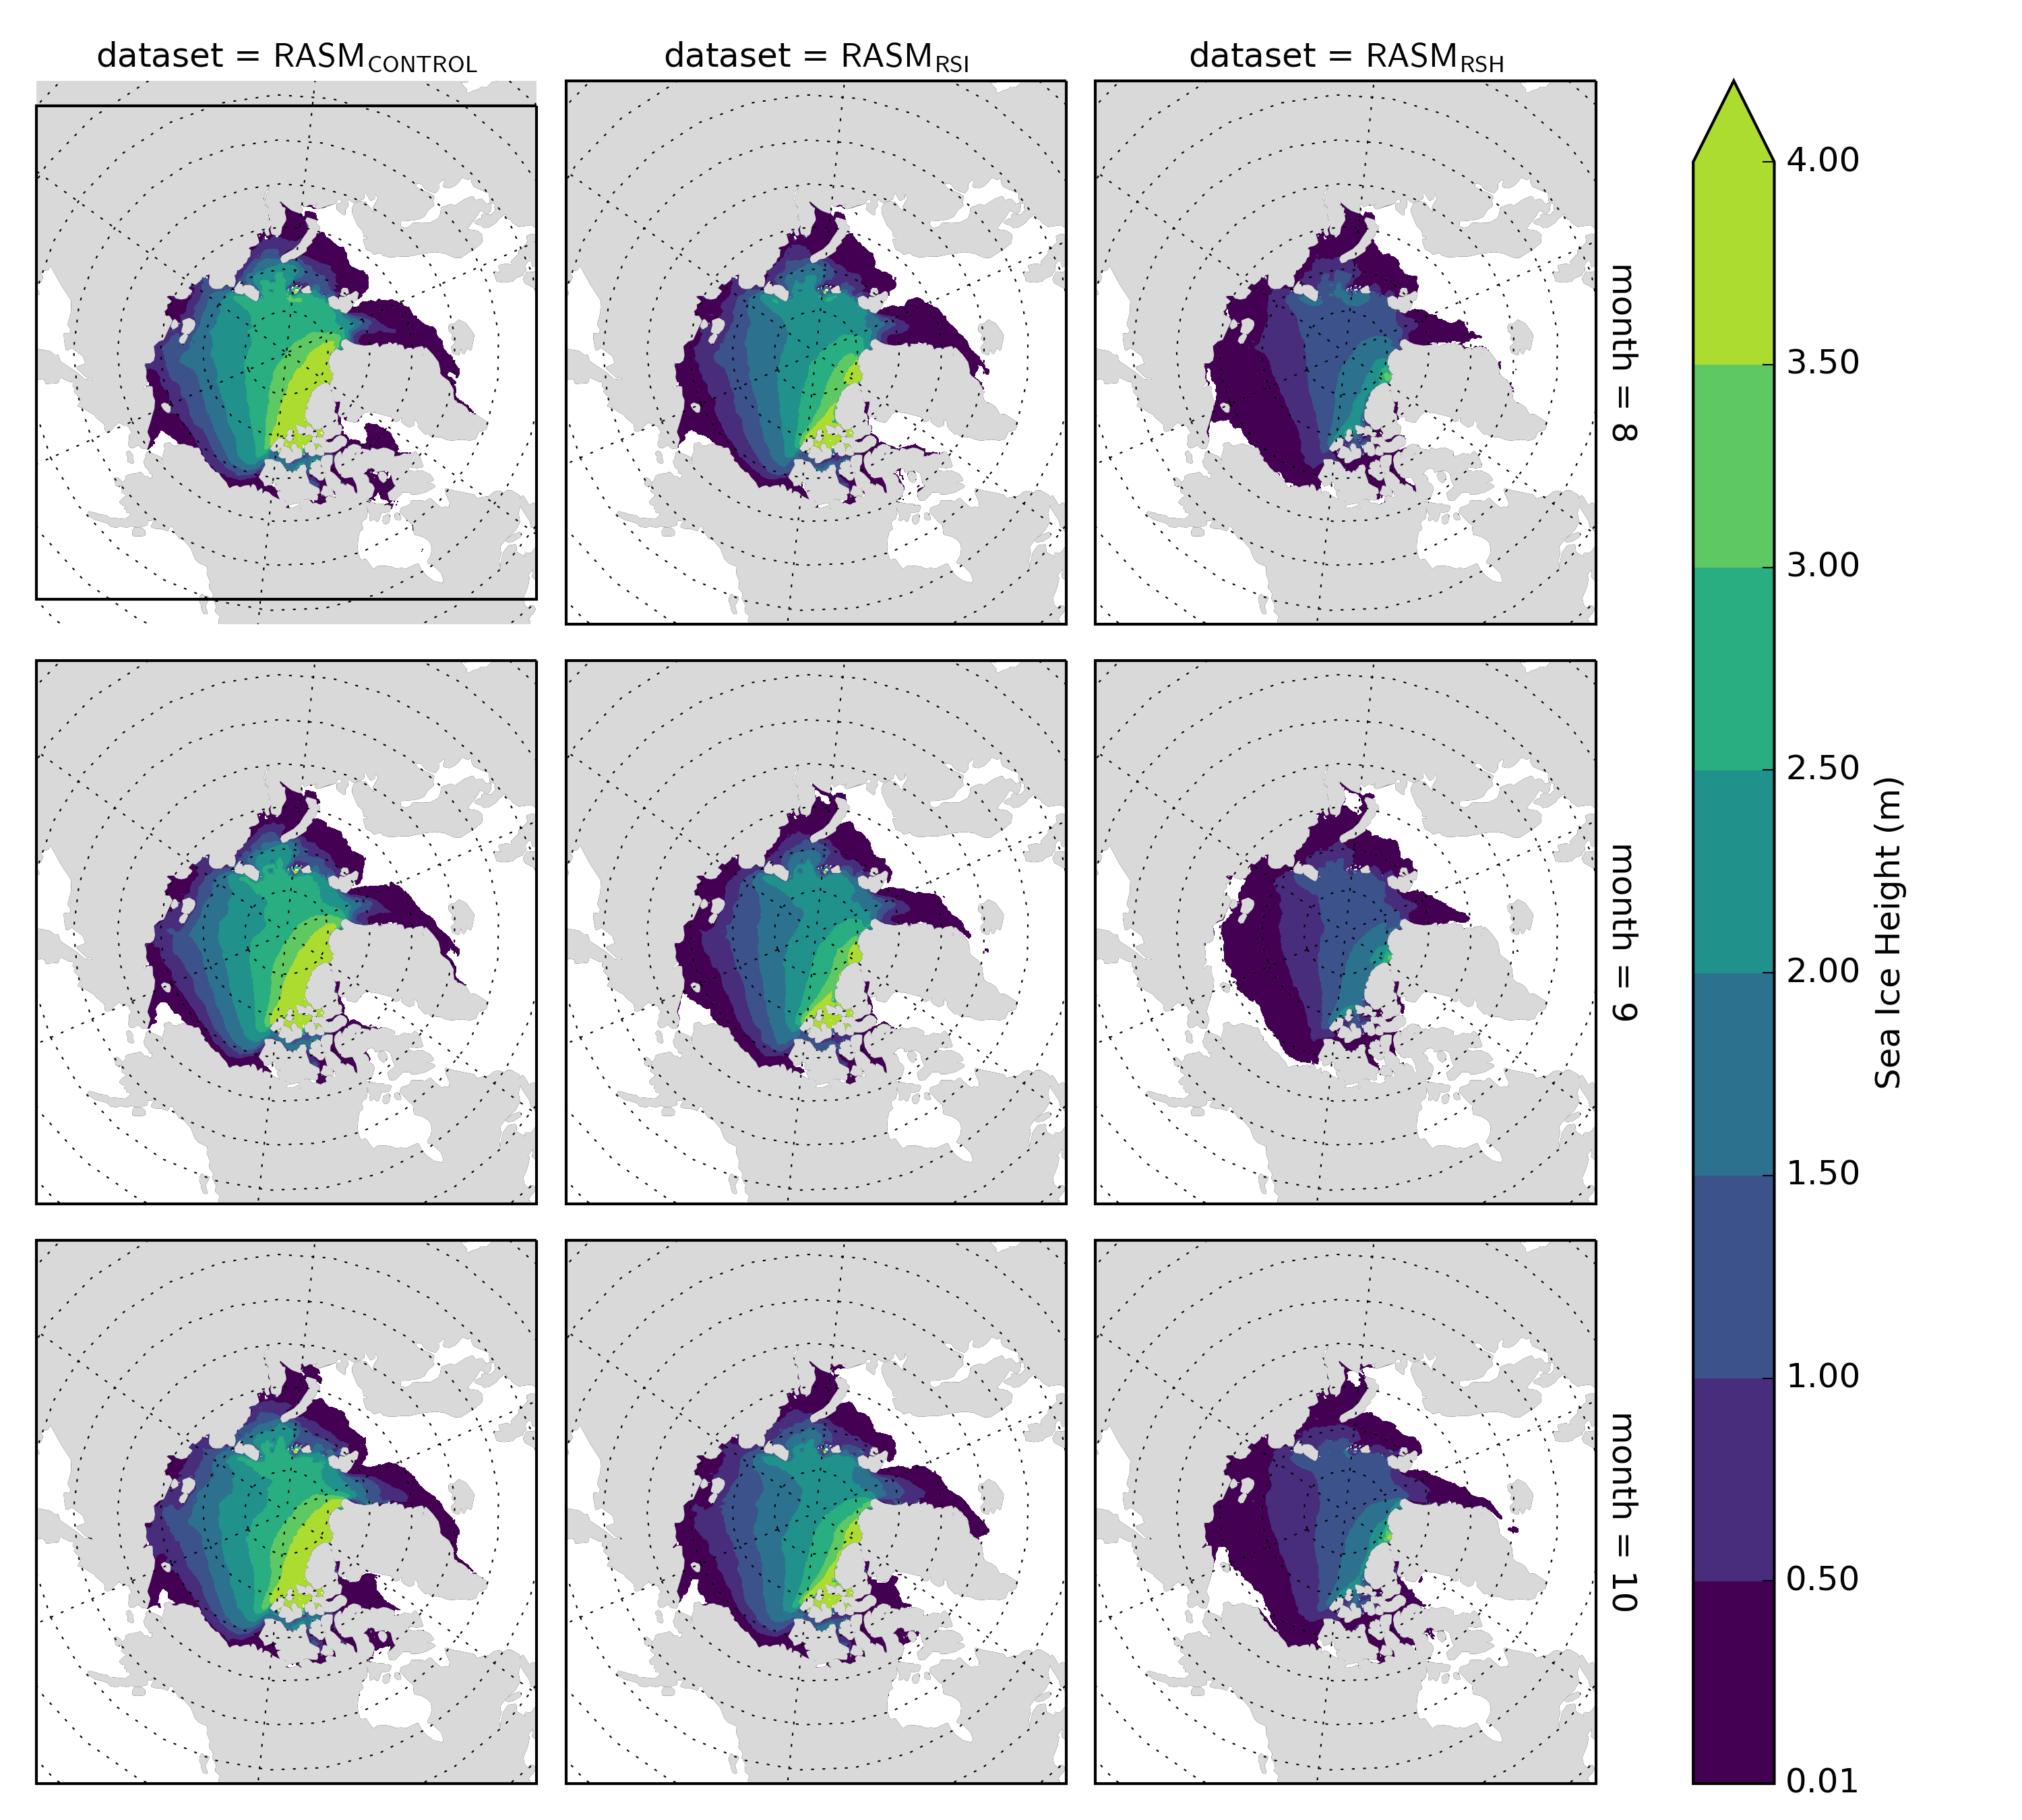
\includegraphics[width=16cm,keepaspectratio]{seaice_height}
    \caption{RASM simulated fall season sea ice heights. Time period: 1985-2014.}
    \label{fig:sea_ice_height_sup}
\end{figure}

\clearpage
\begin{figure}
    \centering
    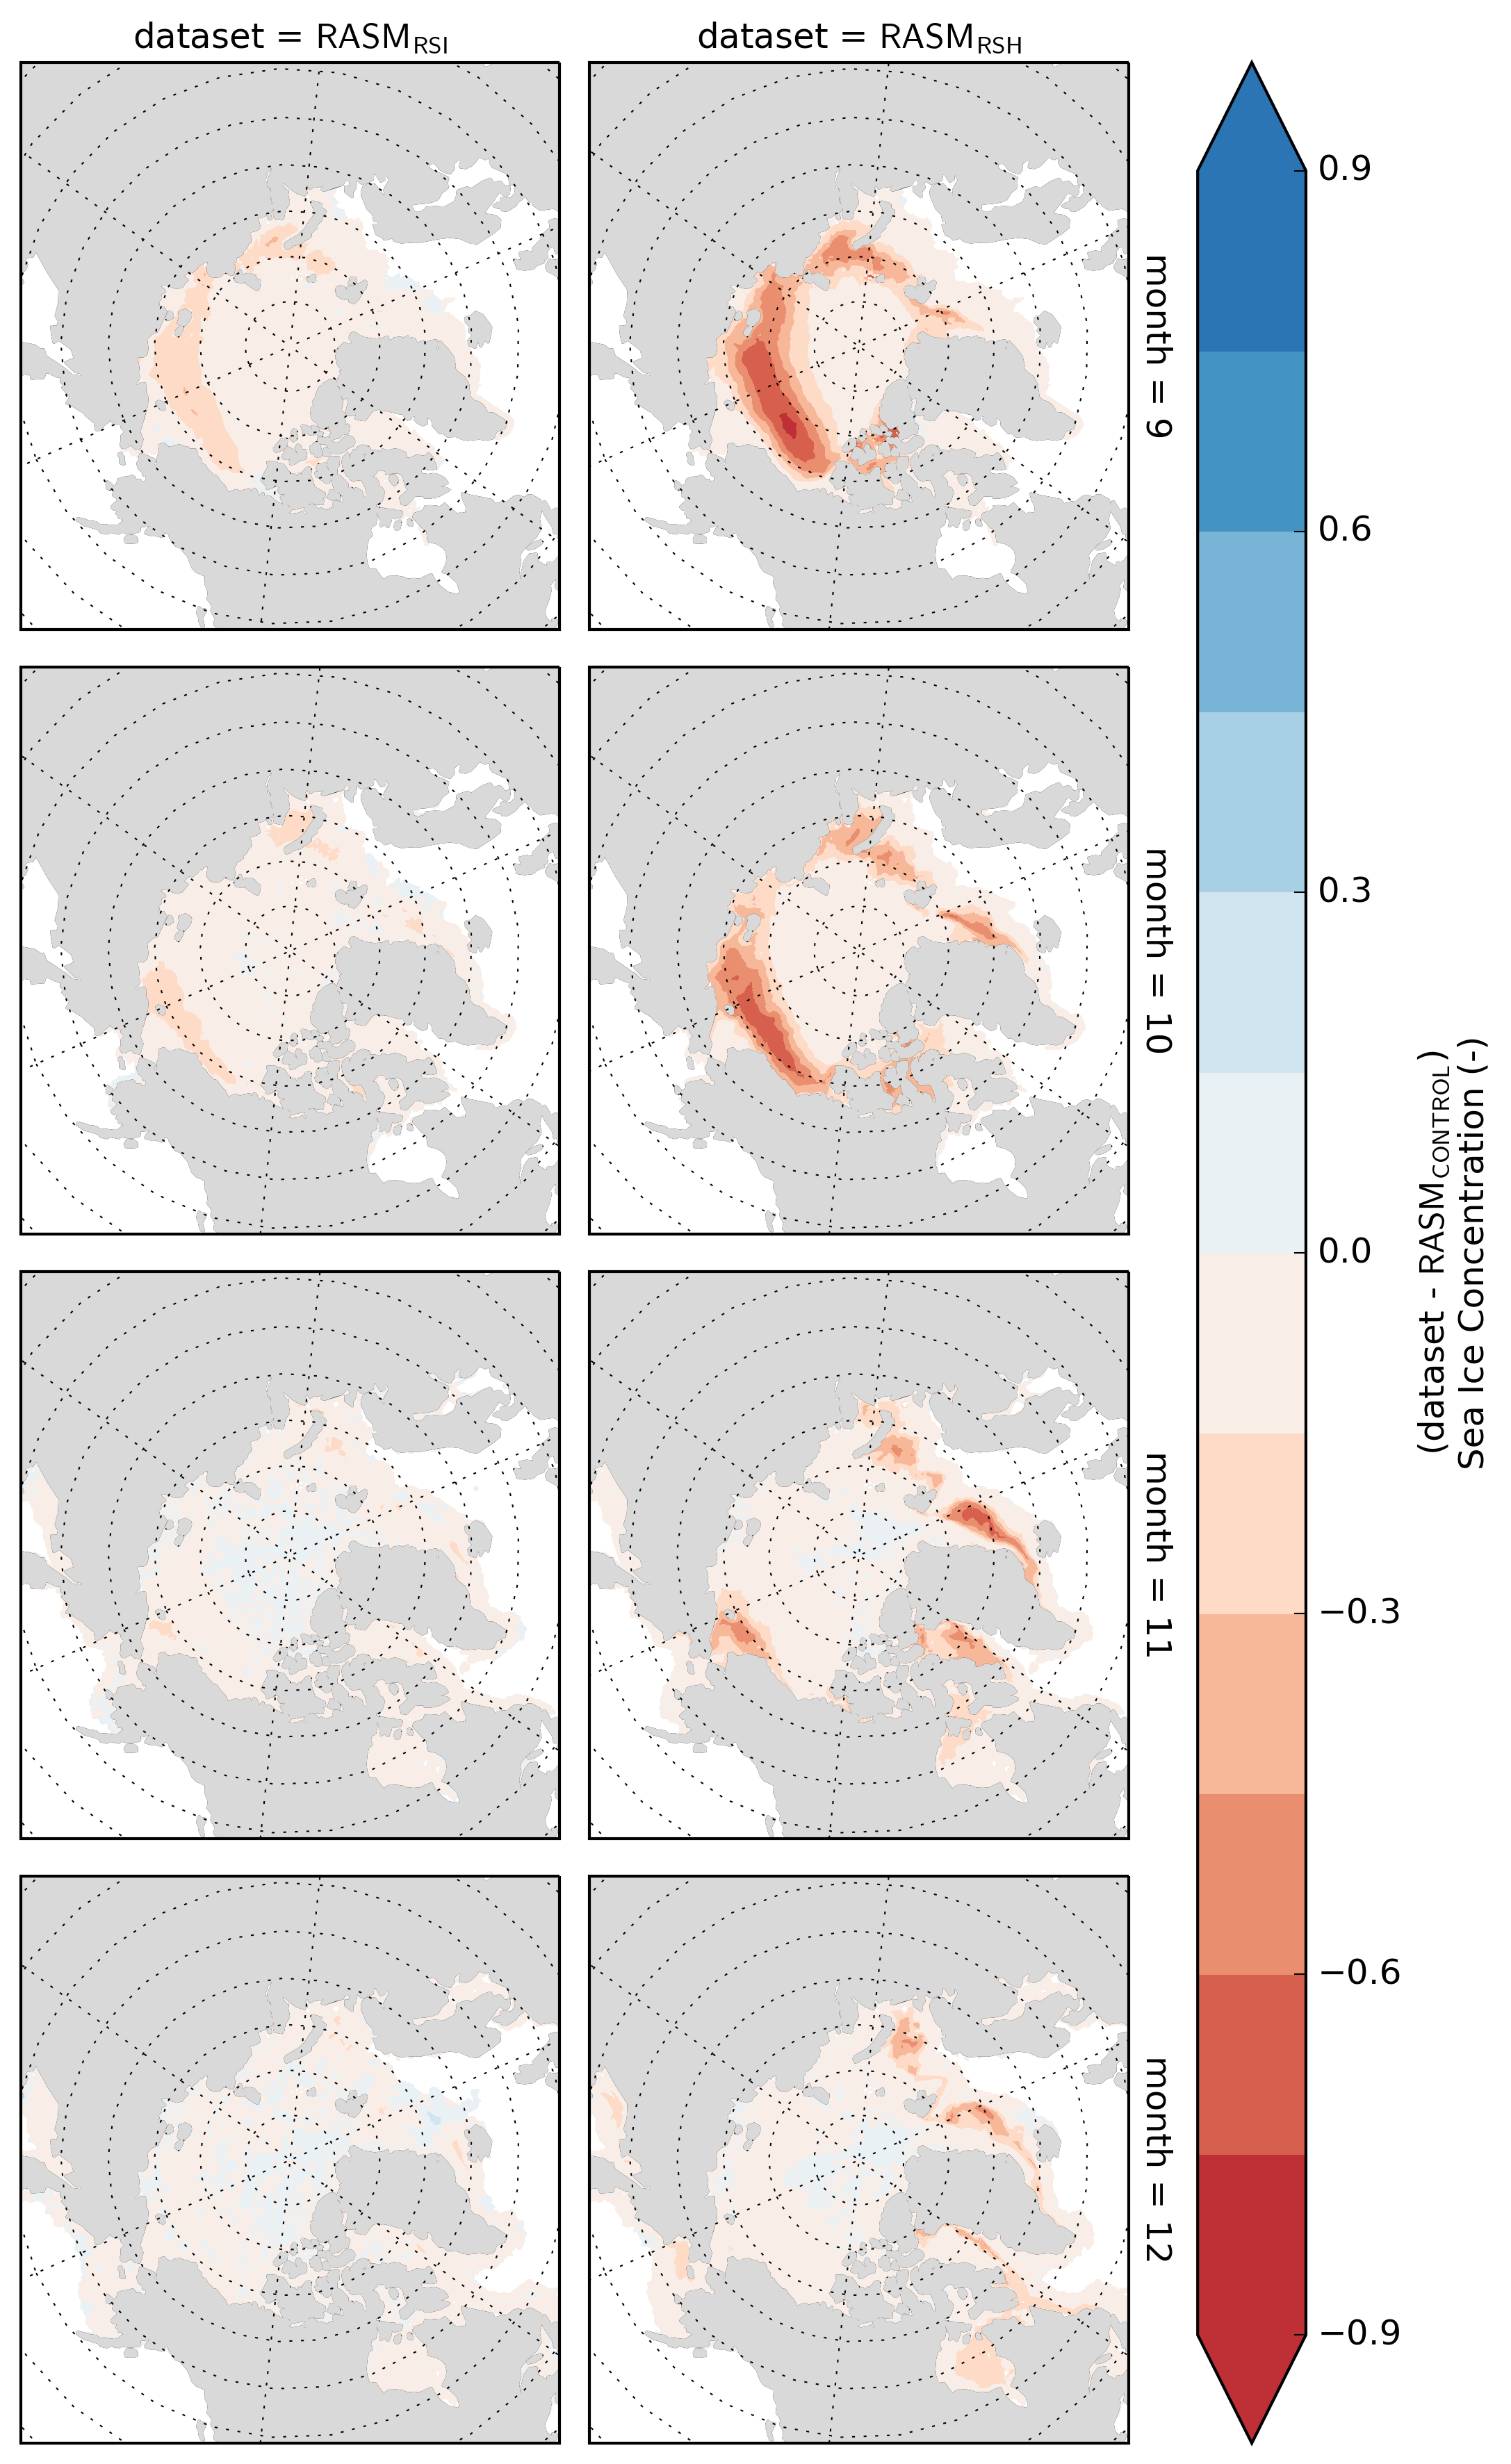
\includegraphics[width=12cm,keepaspectratio]{fall_seaice_concentration_changes}
    \caption{Changes in RASM simulated fall season sea ice concentrations relative to $RASM_{CONTROL}$.
    Time period: 1985-2014.}
    \label{fig:sea_ice_conc_sup}
\end{figure}

\clearpage
\begin{figure}
    \centering
    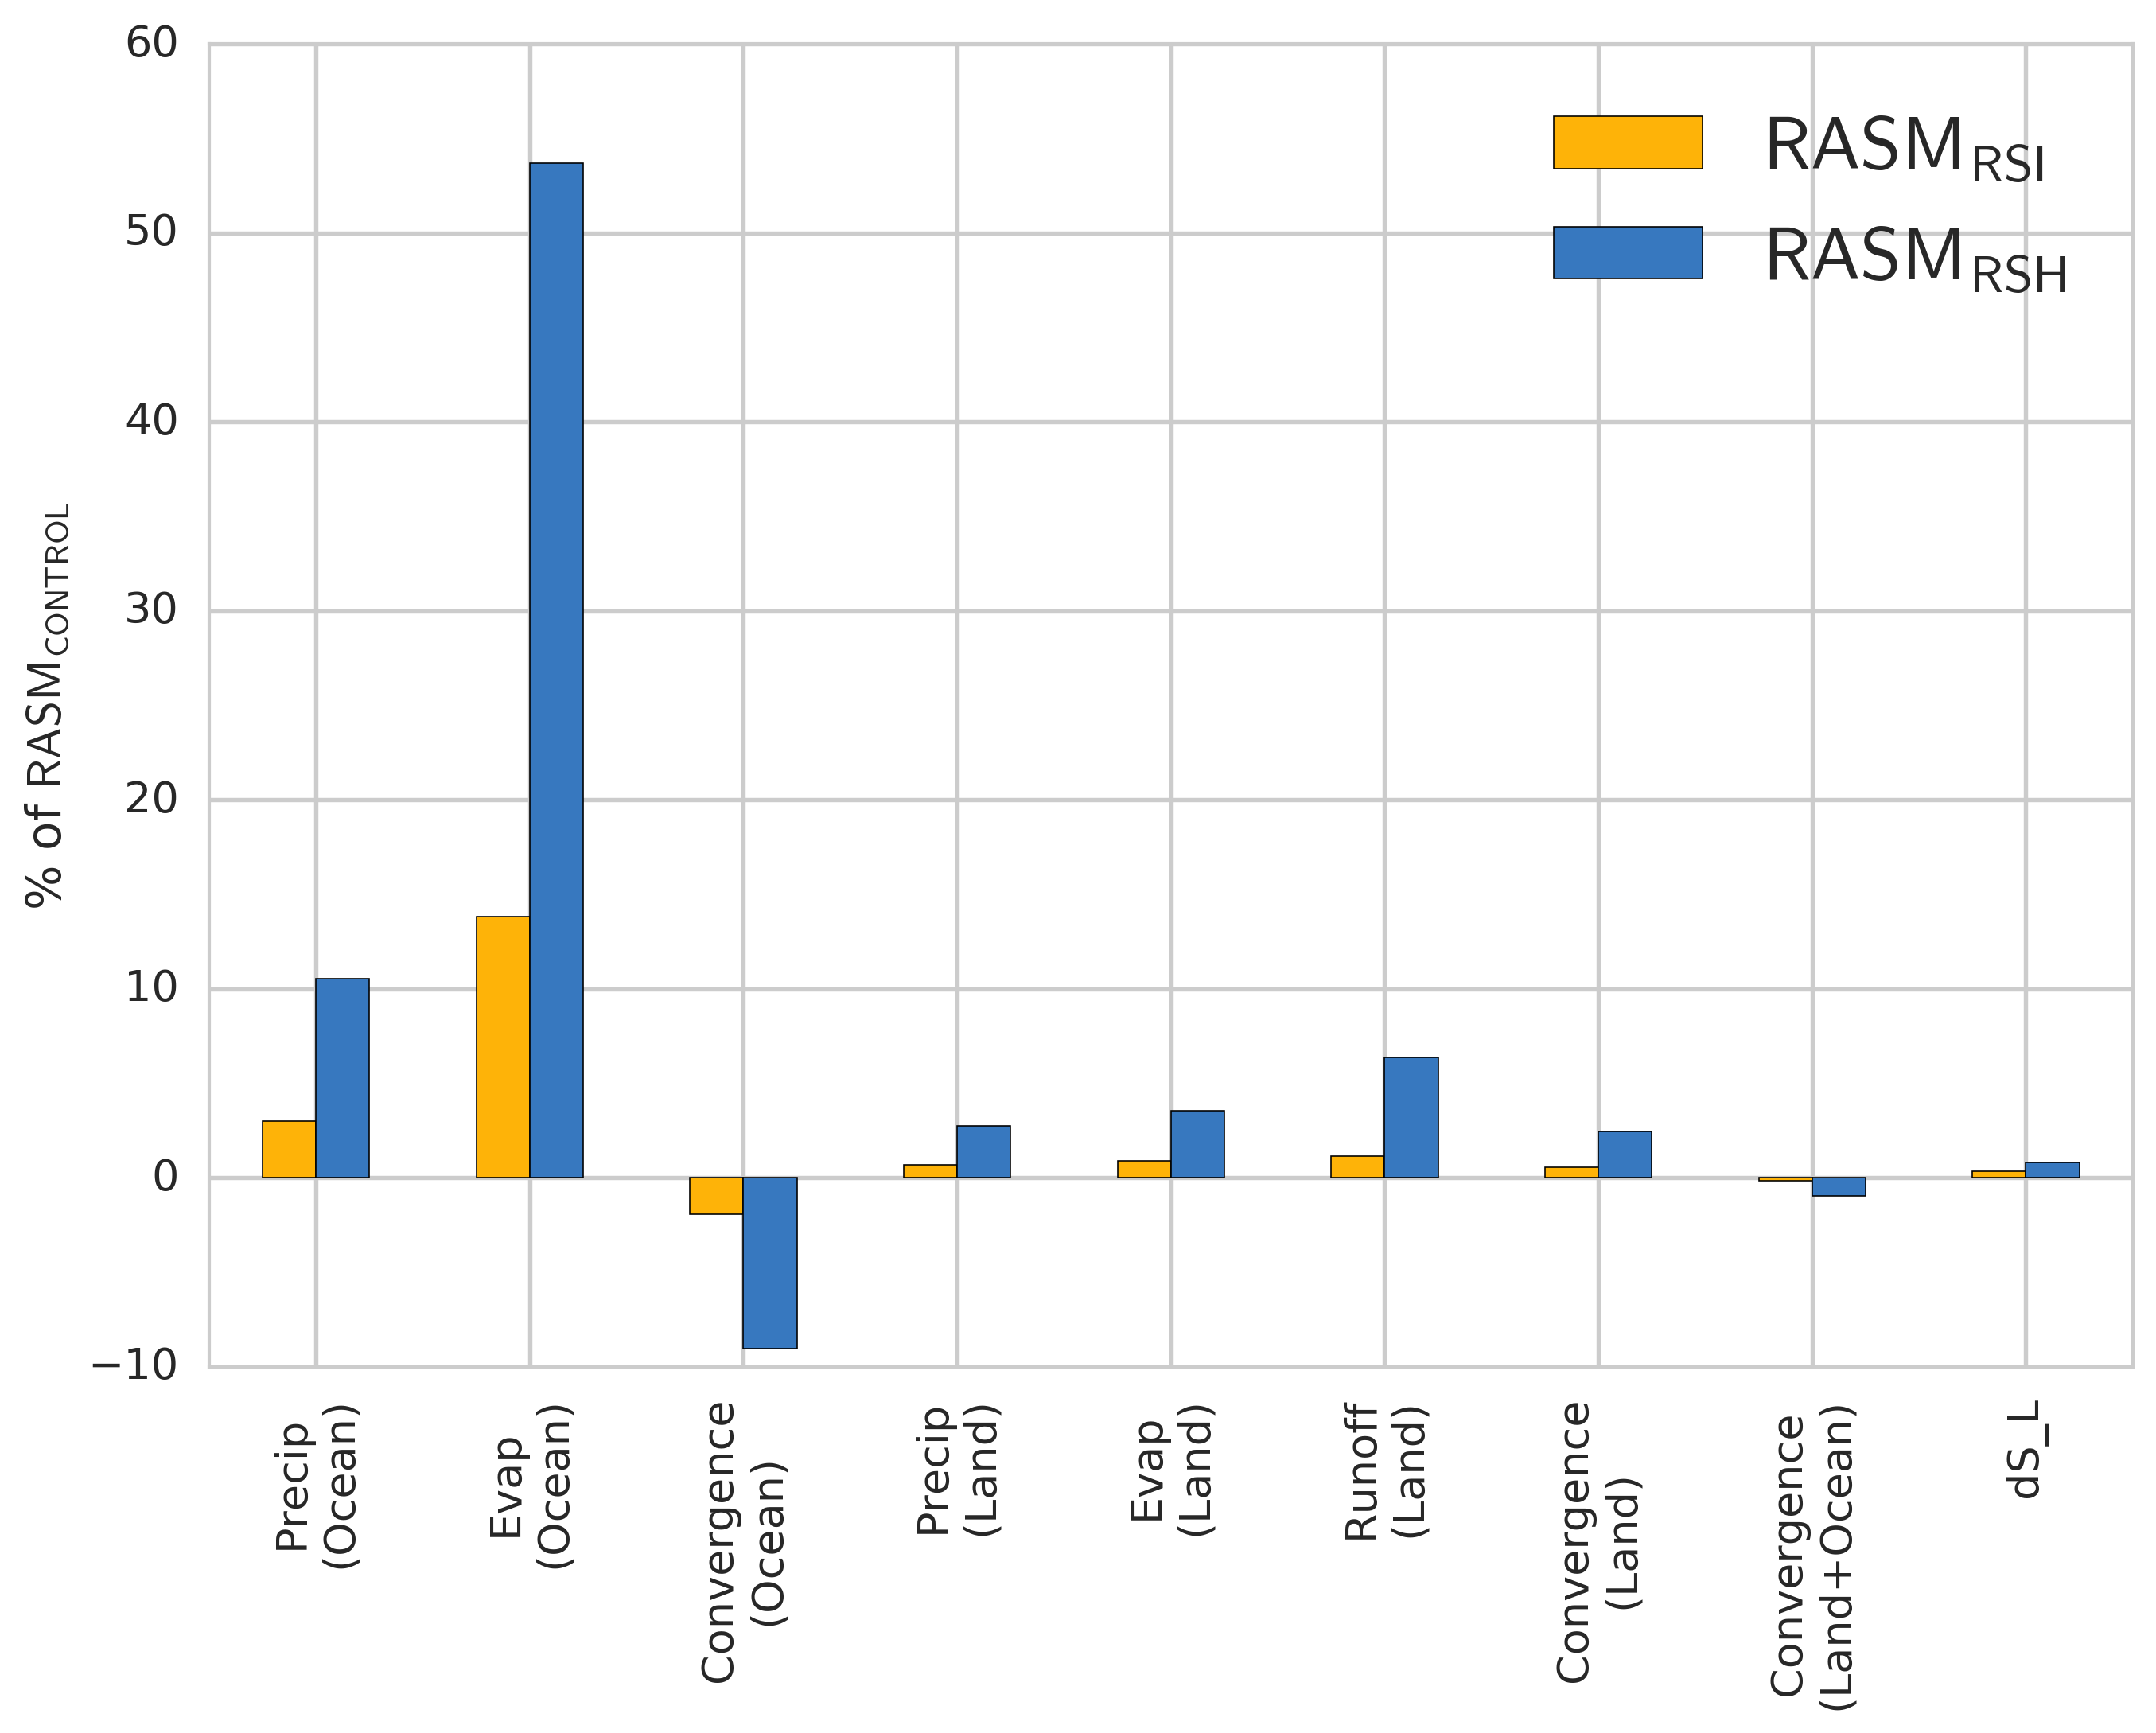
\includegraphics[width=16cm,keepaspectratio]{water_budget_relative}
    \caption{Percent change in fall season water budget fluxes and states relative to $RASM_{CONTROL}$.
    Time period: 1990-2010.}
    \label{fig:relative_fwb_change_sup}
\end{figure}

\clearpage
\section{Tables}

\clearpage
\begin{table}[]
\centering
\caption{Freshwater budget fluxes and standard deviations for the fall season (August-October).}
\label{table:fresh_budget}
\resizebox{8cm}{!}{
\begin{tabular}{|l|l|l|l|l|}
\hline
\textbf{Mask} & \textbf{Variable} & \textbf{Simulation} & \textbf{Mean ($km^3$)} & \textbf{Stdev. ($km^3$)} \\ \hline
Land          & P                 & $RASM_{CONTROL}$    & 2503.59243          & 101.8094554           \\ \hline
Land          & P                 & $RASM_{RSI}$        & 2530.002202         & 103.9974336           \\ \hline
Land          & P                 & $RASM_{RSH}$        & 2565.073088         & 117.3909119           \\ \hline
Land          & E                 & $RASM_{CONTROL}$    & 1293.485951         & 45.1122144            \\ \hline
Land          & E                 & $RASM_{RSI}$        & 1303.650851         & 49.70436952           \\ \hline
Land          & E                 & $RASM_{RSH}$        & 1321.819028         & 49.20729849           \\ \hline
Land          & P-E               & $RASM_{CONTROL}$    & 1210.106479         & 82.0241419            \\ \hline
Land          & P-E               & $RASM_{RSI}$        & 1226.351351         & 93.98460921           \\ \hline
Land          & P-E               & $RASM_{RSH}$        & 1243.254059         & 95.9960839            \\ \hline
Land          & Q                 & $RASM_{CONTROL}$    & 559.7241573         & 43.36381917           \\ \hline
Land          & Q                 & $RASM_{RSI}$        & 565.5626557         & 40.40825329           \\ \hline
Land          & Q                 & $RASM_{RSH}$        & 584.0855527         & 49.72393735           \\ \hline
Land          & P-E-Q             & $RASM_{CONTROL}$    & 650.3823216         & 60.51184041           \\ \hline
Land          & P-E-Q             & $RASM_{RSI}$        & 660.7886949         & 71.67533007           \\ \hline
Land          & P-E-Q             & $RASM_{RSH}$        & 659.1685068         & 64.44975729           \\ \hline
Ocean         & P                 & $RASM_{CONTROL}$    & 989.9575978         & 78.69062911           \\ \hline
Ocean         & P                 & $RASM_{RSI}$        & 1017.003843         & 83.61356705           \\ \hline
Ocean         & P                 & $RASM_{RSH}$        & 1052.348524         & 71.5315201            \\ \hline
Ocean         & E                 & $RASM_{CONTROL}$    & 252.6109753         & 29.83292286           \\ \hline
Ocean         & E                 & $RASM_{RSI}$        & 291.0537803         & 34.42014409           \\ \hline
Ocean         & E                 & $RASM_{RSH}$        & 374.7583967         & 39.50685547           \\ \hline
Ocean         & P-E               & $RASM_{CONTROL}$    & 737.3466225         & 86.55638039           \\ \hline
Ocean         & P-E               & $RASM_{RSI}$        & 725.9500632         & 90.2994341            \\ \hline
Ocean         & P-E               & $RASM_{RSH}$        & 677.5901273         & 87.56230672           \\ \hline
Land + Ocean  & P                 & $RASM_{CONTROL}$    & 3493.432614         & 137.5820565           \\ \hline
Land + Ocean  & P                 & $RASM_{RSI}$        & 3546.885602         & 132.816372            \\ \hline
Land + Ocean  & P                 & $RASM_{RSH}$        & 3617.29704          & 137.8388675           \\ \hline
Land + Ocean  & E                 & $RASM_{CONTROL}$    & 1546.054889         & 57.0214646            \\ \hline
Land + Ocean  & E                 & $RASM_{RSI}$        & 1594.658888         & 70.17793891           \\ \hline
Land + Ocean  & E                 & $RASM_{RSH}$        & 1696.525605         & 69.88332959           \\ \hline
Land + Ocean  & P-E               & $RASM_{CONTROL}$    & 1947.377725         & 125.1580229           \\ \hline
Land + Ocean  & P-E               & $RASM_{RSI}$        & 1952.226714         & 117.7513781           \\ \hline
Land + Ocean  & P-E               & $RASM_{RSH}$        & 1920.771434         & 125.8264945           \\ \hline
\end{tabular}
}
\end{table}

\end{document}
